% a mashup of hipstercv, friggeri and twenty cv
% https://www.latextemplates.com/template/twenty-seconds-resumecv
% https://www.latextemplates.com/template/friggeri-resume-cv

% !TeX program = xelatex 

\documentclass[lighthipster]{simplehipstercv}
% available options are: darkhipster, lighthipster, pastel, allblack, grey, verylight, withoutsidebar
% withoutsidebar
\usepackage[utf8]{inputenc}
\usepackage[default]{raleway}
\usepackage[margin=1cm, a4paper]{geometry}

% 支持中文的设置
\usepackage{xeCJK}
\usepackage{fontspec}
\setCJKmainfont[ItalicFont=思源宋体,BoldFont=SourceHanSerifSC-Bold]{Source Han Serif SC}
\newcommand{\KaiTi}{\CJKfontspec{楷体}}%用命令\fzkaiti调用方正楷体简体

%------------------------------------------------------------------ Variablen

\newlength{\rightcolwidth}
\newlength{\leftcolwidth}
\setlength{\leftcolwidth}{0.23\textwidth}
\setlength{\rightcolwidth}{0.75\textwidth}

%------------------------------------------------------------------
\title{New Simple CV}
\author{\LaTeX{} Ninja}
\date{June 2019}

\pagestyle{empty}
\begin{document}
	
	
	\thispagestyle{empty}
	%-------------------------------------------------------------
	
	\section*{Start}
	
	\simpleheader{headercolour}{王}{升平}{软件部副经理}{white}
	
	
	
	%------------------------------------------------
	
	% this has to be here so the paracols starts..
	\subsection*{}
	\vspace{4em}
	
	\setlength{\columnsep}{1.5cm}
	\columnratio{0.23}[0.75]
	\begin{paracol}{2}
		\hbadness5000
		%\backgroundcolor{c[1]}[rgb]{1,1,0.8} % cream yellow for column-1 %\backgroundcolor{g}[rgb]{0.8,1,1} % \backgroundcolor{l}[rgb]{0,0,0.7} % dark blue for left margin
		
		\paracolbackgroundoptions
		
		% 0.9,0.9,0.9 -- 0.8,0.8,0.8
		
		
		\footnotesize
		{\setasidefontcolour
			\flushright
			\begin{center}
				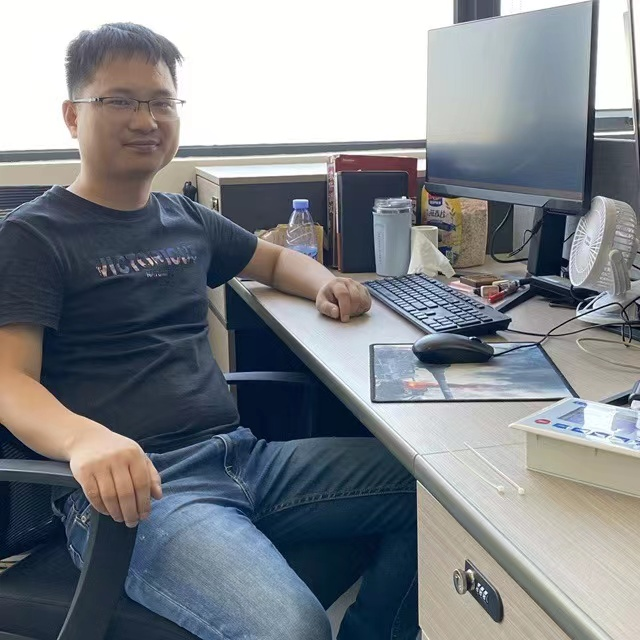
\includegraphics[width=\linewidth]{ShowMe.jpg}
			\end{center}
			\bigskip
			
			\bg{cvgreen}{white}{关于我}\\[0.5em]
			
			{\footnotesize
				\lorem\lorem\lorem}
			\bigskip
			
			\bg{cvgreen}{white}{个人信息} \\[0.5em]
			王升平
			
			籍贯: 湖北 
			
			1989
			
			\bigskip
			
			\bg{cvgreen}{white}{Areas of specialization} \\[0.5em]
			
			Privateering ~•~ Bucaneering ~•~ Parler ~•~ Rum
			
			\bigskip
			
			
			
			\bigskip
			
			\bg{cvgreen}{white}{Interests}\\[0.5em]
			
			\lorem
			\bigskip
			
			\bg{cvgreen}{white}{Interests}\\[0.5em]
			
			\texttt{R} ~/~ \texttt{Android} ~/~ \texttt{Linux}
			
			\texttt{R} ~/~ \texttt{Android} ~/~ \texttt{Linux}
			
			\texttt{R} ~/~ \texttt{Android} ~/~ \texttt{Linux}
			
			\vspace{4em}
			
			\infobubble{\faGithub}{cvgreen}{white}{thinct}
			
			\phantom{turn the page}
			
			\phantom{turn the page}
		}
		%-----------------------------------------------------------
		\switchcolumn
		
		\small
		\section*{公司简历}
		
		\begin{tabular}{r| p{0.5\textwidth} c}
			\cvevent{2021--2023}{东莞市雷宇激光设备有限公司}{Lead}{East Indies \color{cvred}}{Finally got the goddamn ship back.\lorem\lorem\lorem}{logo_TL.png} \\
			\cvevent{2012--2021}{广东省奥普特股份有限公司(股票号:688686)}{Lead}{Tortuga \color{cvred}}{Found a secret treasure, lost the ship. \lorem\lorem}{logo_OPT.pdf}
		\end{tabular}
		\vspace{3em}
		
		\begin{minipage}[t]{0.35\textwidth}
			\section*{Degrees}
			\begin{tabular}{r p{0.6\textwidth} c}
				\cvdegree{1710}{Captain}{Certified}{Tortuga Uni \color{headerblue}}{}{disney.png} \\
				\cvdegree{1715}{Bucaneering}{M.A.}{London \color{headerblue}}{}{medal.jpeg} \\
				\cvdegree{1720}{Bucaneering}{B.A.}{London \color{headerblue}}{}{medal.jpeg}
			\end{tabular}
		\end{minipage}\hfill
		\begin{minipage}[t]{0.3\textwidth}
			\section*{编程技能}
			\begin{tabular}{r @{\hspace{0.5em}}l}
				\bg{skilllabelcolour}{iconcolour}{VC++} &  \barrule{0.4}{0.5em}{cvpurple}\\
				\bg{skilllabelcolour}{iconcolour}{C++} & \barrule{0.55}{0.5em}{cvgreen} \\
				\bg{skilllabelcolour}{iconcolour}{Qt} & \barrule{0.5}{0.5em}{cvpurple} \\
				\bg{skilllabelcolour}{iconcolour}{WinDbg} & \barrule{0.25}{0.5em}{cvpurple} \\
				\bg{skilllabelcolour}{iconcolour}{Python} & \barrule{0.1}{0.5em}{cvpurple} \\
			\end{tabular}
		\end{minipage}
		
		\section*{产品简介}
		\begin{tabular}{r| p{0.5\textwidth} c}
			\cvevent{2022--2023}{Laser Maker V2.0}{Lead}{East Indies \color{cvred}}{Finally got the goddamn ship back. \lorem}{disney.png} \\
			\cvevent{2012--2021}{SciSmart V2.0/V3.0}{Bucaneering}{Tortuga \color{cvred}}{This and that. The usual, aye?  \lorem}{medal.jpeg} \\
		\end{tabular}
		\vspace{3em}
		
		\begin{minipage}[t]{0.3\textwidth}
			\section*{Certificates \& Grants}
			\begin{tabular}{>{\footnotesize\bfseries}r >{\footnotesize}p{0.55\textwidth}}
				1708 & Captain's Certificates \\
				1710 & Travel grant \\
				1715--1716 & Grant from the Pirate's Company
			\end{tabular}
			\bigskip
			
			\section*{Languages}
			\begin{tabular}{l | ll}
				\textbf{English} & C2 & {\phantom{x}\footnotesize mother tongue} \\
				\textbf{French} & C2 & \pictofraction{\faCircle}{cvgreen}{3}{black!30}{1}{\tiny} \\
				\textbf{Spanish} & C2 & \pictofraction{\faCircle}{cvgreen}{1}{black!30}{3}{\tiny} \\
				\textbf{Italian} & C2 & \pictofraction{\faCircle}{cvgreen}{3}{black!30}{1}{\tiny}
			\end{tabular}
			\bigskip
			
		\end{minipage}\hfill
		\begin{minipage}[t]{0.3\textwidth}
			\section*{Publications}
			\begin{tabular}{>{\footnotesize\bfseries}r >{\footnotesize}p{0.7\textwidth}}
				1729 & \emph{How I almost got killed by Lady Swan}, Tortuga Printing Press. \\
				1720 & ``Privateering for Beginners'', in: \emph{The Pragmatic Pirate} (1/1720).
			\end{tabular}
			\bigskip
			
			\section*{Talks}
			\begin{tabular}{>{\footnotesize\bfseries}r >{\footnotesize}p{0.6\textwidth}}
				Nov. 1726 & ``How I lost my ship (\& and how to get it back)'', at: \emph{Annual Pirate's Conference} in Tortuga, Nov. 1726.
			\end{tabular}
		\end{minipage}
		
		
		
		
		
		
		\vfill{} % Whitespace before final footer
		
		%----------------------------------------------------------------------------------------
		%	FINAL FOOTER
		%----------------------------------------------------------------------------------------
		\setlength{\parindent}{0pt}
		\begin{minipage}[t]{\rightcolwidth}
			\begin{center}\fontfamily{\sfdefault}\selectfont \color{black!70}
				{\icon{\faMapMarker}{cvgreen}{} GuangDong/DongGuan \icon{\faPhone}{cvgreen}{} 13265599720 \icon{\faAt}{cvgreen}{} \protect\url{thinct_123@foxmail.com}
				}
			\end{center}
		\end{minipage}
		
	\end{paracol}
	
\end{document}
